\section{Experiments}
\label{sec:empirical} 
We start by studying the impact of reflow on toy examples. 
After that, 
we demonstrate that with multiple times of reflow, rectified flow achieves state-of-the-art performance on CIFAR-10. 
Moreover, it can also generate high-quality images on high-resolution image datasets. 
Going beyond unconditioned image generation, we apply our method to unpaired image-to-image translation tasks to generate visually high-quality image pairs. 


\paragraph{Algorithm} 
We follow the procedure in Algorithm~\ref{alg:cap}. 
We start with drawing $(X_0,X_1)\sim \tg_0 \times \tg_1$ and use it to get the first rectified flow $\vv Z^1$ by minimizing \eqref{equ:mainf}.
The second rectified flow $\vv Z^2$ is obtained by the same procedure except with the data replaced by the draws from $(Z_0^1,Z_1^1)$, 
obtained by simulating the first rectified flow $\vv Z^1$. This process is repeated for $k$ times to get the \emph{$k$-rectified flow} $\vv Z^k$.
Finally, we can further distill the  \emph{$k$-rectified flow} $\vv Z^k$  into a one step model $z_1= z_0 +  v(z_0, 0)$ by fitting it on draws from $(Z_0^k, Z_1^k)$. 

By default, the ODEs 
are simulated using the vanilla Euler method with constant step size $1/N$ for $N$ steps, that is,  $\hat Z_{t+1/N} = \hat Z_{t} + v(\hat Z_{t}, t)/N$ for $t \in\{0,\ldots, N\}/N$. 
We use the Runge-Kutta method of order 5(4) from Scipy 
\citep{2020SciPy-NMeth}, denoted as RK45, 
which adaptively decide the step size and number of steps $N$ based on  user-specified relative and absolute tolerances.  
In our experiments, we stick to the same parameters as~\cite{song2020score}.


\subsection{Toy Examples}
\label{sec:toy}
To accurately illustrate the theoretical properties,
we use the non-parametric estimator $v^{X,h}(z,t)$ in \eqref{equ:npfunc} in the toy examples in Figure~\ref{fig:twodotstoy}, \ref{fig:toystar}, \ref{fig:gauss2dots}, \ref{fig:speedtoy}.  
In practice, we approximate the expectation in \eqref{equ:npfunc} an nearest neighbor estimator: given a sample 
$\{x_0\datai, x_1\datai\}_i$ 
drawn from $(X_0,X_1)$, 
we estimate $v^X$ by 
\bb 
v^{X,h}(z,t) \approx \!\!\! \sum_{i\in \mathrm{knn}(z, m)}\!\!\!  \frac{x_1\datai - z}{1-t} \omega_h(x_t\datai, z)~~/\!\!\!
\sum_{i\in \mathrm{knn}(z, m)} \!\!\!\!\! \omega_h(x_t\datai, z), 
&&
x_t\datai =t x_1\datai + (1-t) x_0\datai, 
\ee 
where $\mathrm{knn}(z, m)$ 
denotes the top $m$ nearest neighbors of $z$ in $\{x_t\datai\}_i$.  
We find that the results are not sensitive to the choice of $m$ and the bandwidth $h$ (see Figure~\ref{fig:smoothness}). 
We use $h = 1$ and $m = 100$ by default.  
The flows are simulated using Euler method
with a constant step size of $1/N$ for $N$ steps.
We use $N=100$ steps unless otherwise specified. %



Alternatively, $v^X$ can be parameterized as a neural network and trained with stochastic gradient descent or Adam. %
Figure \ref{fig:smoothness} shows an example of when $v^X$ is parameterized as an 2-hidden-layer fully connected neural network with 64 neurons in both hidden layers. %
We see that the neural networks fit less perfectly with the linear interpolation trajectories 
(which should be piece-wise linear in this toy example).  
As shown in Figure~\ref{fig:smoothness}, 
we find that enhancing the smoothness of the  neural networks (by increasing the L2 regularization coefficient during training) can help  straighten the flow, in addition to the rectification effect. %





\newcommand{\tmpfsize}{\scriptsize}
\begin{figure}[tbh]
\centering
\scalebox{1}{
\begin{tabular}{cccccc}
\tmpfsize  1-Rectified Flow & \tmpfsize  2-Rectified Flow  & \tmpfsize  3-Rectified Flow  & 
\tmpfsize  1-Rectified Flow  & \tmpfsize  2-Rectified Flow   &\tmpfsize   3-Rectified Flow   \\
\raisebox{1em}{\rotatebox{90}{\tmpfsize{L2 Penalty}=0}}
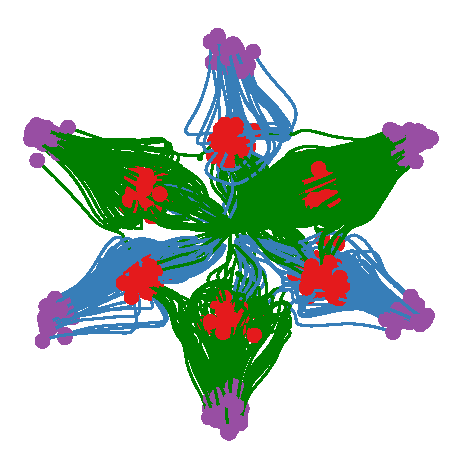
\includegraphics[width=.14\textwidth]{arxiv_figures/flow_wd0.pdf}
& 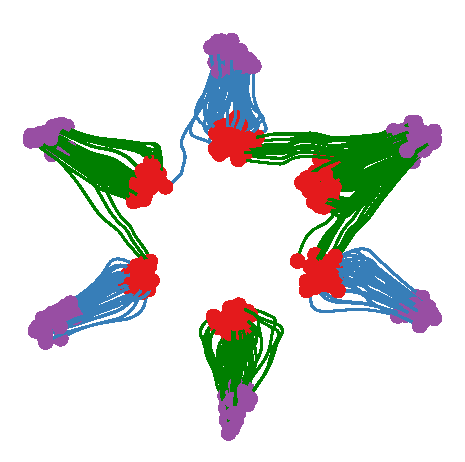
\includegraphics[width=.14\textwidth]{arxiv_figures/reflow_wd0.pdf} & 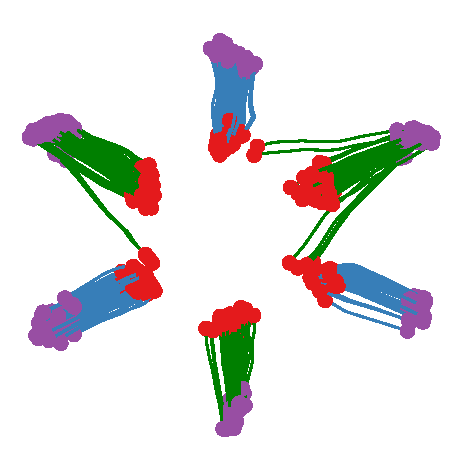
\includegraphics[width=.14\textwidth]{arxiv_figures/reflow2_wd0.pdf} & 
\raisebox{1.8em}{\rotatebox{90}{\tmpfsize{$h=0.01$}}}
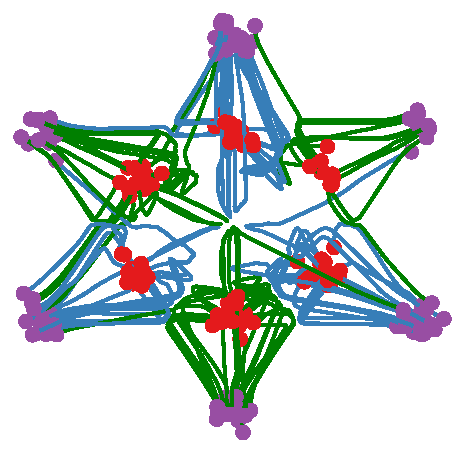
\includegraphics[width=.14\textwidth]{arxiv_figures/reflow_kernel_h0.01.pdf}& 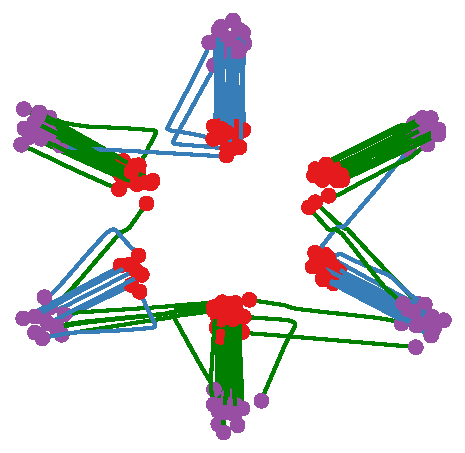
\includegraphics[width=.14\textwidth]{arxiv_figures/reflow_kernel1_h0.01.pdf} & 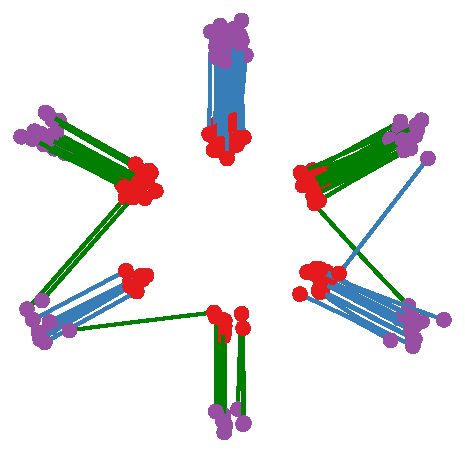
\includegraphics[width=.14\textwidth]{arxiv_figures/reflow_kernel2_h0.01.pdf} \\
\raisebox{.5em}{\rotatebox{90}{\tmpfsize{L2 Penalty$=0.01$}}}
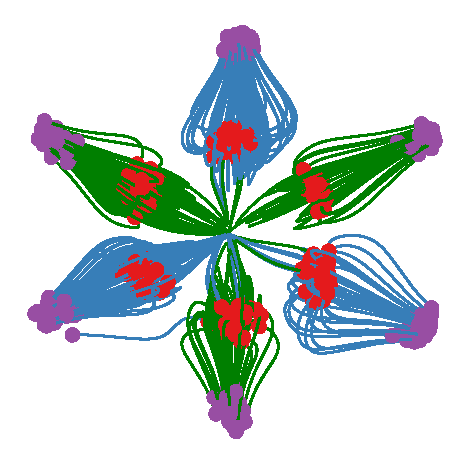
\includegraphics[width=.14\textwidth]{arxiv_figures/flow_wd0.01.pdf}
& 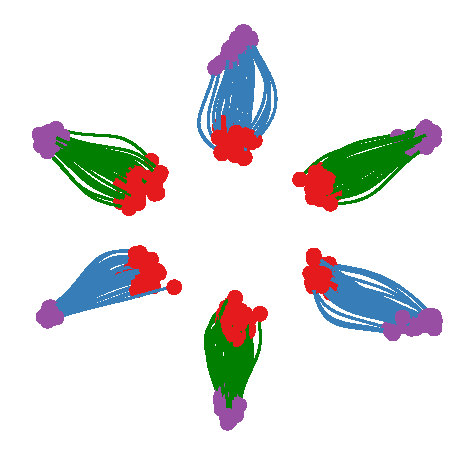
\includegraphics[width=.14\textwidth]{arxiv_figures/reflow_wd0.01.pdf} & 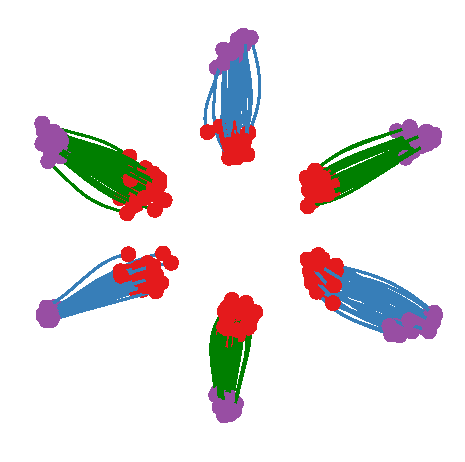
\includegraphics[width=.14\textwidth]{arxiv_figures/reflow1_wd0.01.pdf} &
\raisebox{1.2em}{\rotatebox{90}{\tmpfsize{$h=1$}}}
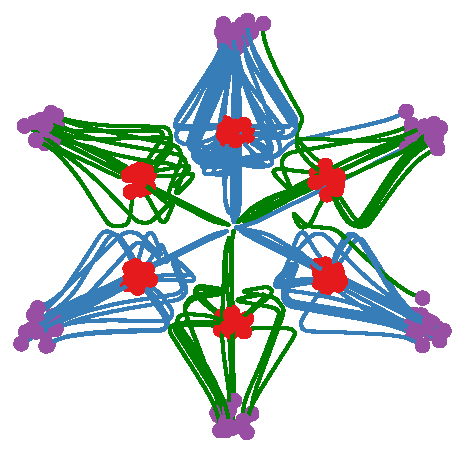
\includegraphics[width=.14\textwidth]{arxiv_figures/reflow_kernel_h1.pdf}
& 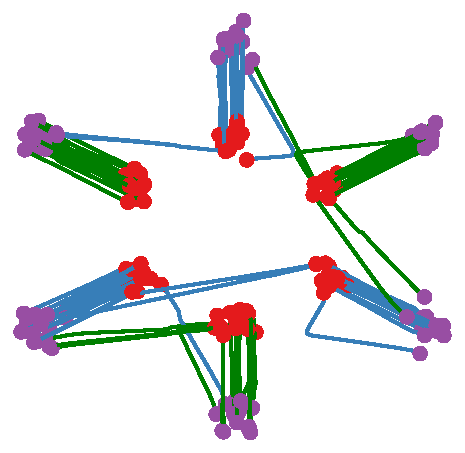
\includegraphics[width=.14\textwidth]{arxiv_figures/reflow_kernel1_h1.pdf} & 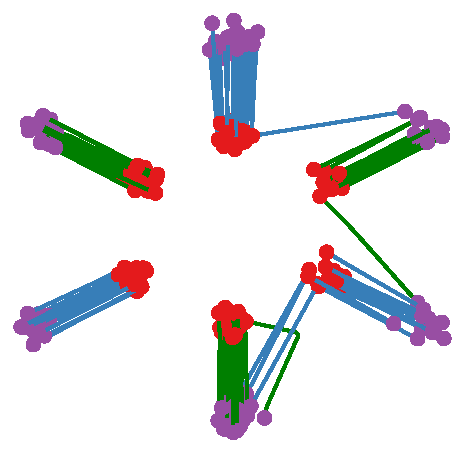
\includegraphics[width=.14\textwidth]{arxiv_figures/reflow_kernel2_h1.pdf} \\

\vspace{-15pt}
\end{tabular}}
\caption{
Rectified flows 
fitted with 
neural networks trained with different L2 penalty (left), and kernel estimator with different bandwidth $h$ (right).  
$\tg_0$: red dots; $\tg_1$: purple dots. 
}
\label{fig:smoothness}
\vspace{-5pt}
\end{figure}

In Figure~\ref{fig:toystar} of Section~\ref{sec:secondintro},  
the straightness is calculated as the empirical estimation of \eqref{equ:straight} based on the simulated trajectories.
The relative transport cost is calculated based on  $\{z_0\datai,z_1\datai\}_{i=1}^n$ drawn from $(Z_0,Z_1)$ by simulating the flow, as $\frac{1}{n}\sum_{i=1}^n \norm{z_1\datai-z_0\datai}^2 - \norm{z_1\dataidx{i^*}-z_0\datai}^2$, where $z_1\dataidx{i^*}$ is the optimal L2 assignment of $z_0\datai$ obtained by solving the discrete L2 optimal transport problem between $\{z_0\datai\}$ and $\{z_1\datai\}$. 
We should 
note that this metric is only useful in low dimensions, as it tends to be identically zero in high dimensional cases 
even $v^X$ is set to be a random neural network.
This misleading phenomenon is what causes  \cite{khrulkov2022understanding} to make the false hypothesis that DDIM yields L2 optimal transport. 


\subsection{Unconditioned Image Generation}
\label{sec:exp:cifar}



We test rectified flow for unconditioned image generation on CIAFR-10 and a number of high resolution datasets. 
The methods are evaluated by the quality of generated images by Fréchet inception distance (FID) and inception score (IS), 
 and the diversity of the generated images by the recall score  following \citep{kynkaanniemi2019improved}.

\paragraph{Experiment settings}
For the purpose of generative modeling, we set $\tg_0$ to be the standard Gaussian distribution and $\tg_1$ the data distribution. 
Our implementation of rectified flow is modified upon the open-source code of ~\citep{song2020score}. %
We adopt the U-Net architecture of DDPM++~\cite{song2020score} for representing the drift $v^X$, 
and report in Table~\ref{tab:cifar10} (a)  and Figure~\ref{fig:cifar} the results of our method and the (sub)-VP ODE from \cite{song2020score} using the same architecture.  
Other recent results using different network architectures are shown in Table~\ref{tab:cifar10} (b) for reference. 
More detailed settings can be found in the Appendix.



\begin{table}[h]
    \centering
    \begin{tabular}{cc} 
    \resizebox{.5\textwidth}{!}{
    \begin{tabular}{lcccc}
        \hline \hline
        Method  & NFE($\downarrow$) & IS ($\uparrow$) & FID ($\downarrow$) & Recall ($\uparrow$) \\  \hline \hline 
        \emph{ODE} &
        \multicolumn{4}{l}{\emph{One-Step Generation (Euler solver, N=1)}} \\
        \hline 
         \textbf{1-Rectified Flow (\emph{+Distill}) } & 1 & 1.13 (\emph{\textbf{9.08}}) & 378 (\emph{6.18}) & 0.0 (\emph{0.45}) \\
        \textbf{2-Rectified Flow (\emph{+Distill}) } & 1 & 8.08 (\emph{9.01}) & 12.21 (\emph{\textbf{4.85}}) & 0.34 (\emph{0.50}) \\
         \textbf{3-Rectified Flow (\emph{+Distill}) } & 1 & 8.47 (\emph{8.79}) & 8.15 (\emph{5.21}) & 0.41 (\emph{\textbf{0.51}}) \\
        VP ODE~\citep{song2020score} (\emph{+Distill}) & 1 & 1.20 (\emph{8.73}) & 451 (\emph{16.23}) & 0.0 (\emph{0.29}) \\
         sub-VP ODE~\citep{song2020score} (\emph{+Distill}) & 1 & 1.21 (\emph{8.80}) & 451 (\emph{14.32}) & 0.0 (\emph{0.35}) \\
         \hline \hline  
         \emph{ODE} & 
          \multicolumn{4}{l}{\emph{Full Simulation (Runge–Kutta (RK45), Adaptive $N$)}} \\ 
        \hline           
         \textbf{1-Rectified Flow} & 127 & \textbf{9.60} & \textbf{2.58} & \textbf{0.57} \\
         \textbf{2-Rectified Flow} & 110 & 9.24 & 3.36 & 0.54 \\
         \textbf{3-Rectified Flow} & 104 & 9.01 & 3.96 & 0.53 \\
        VP ODE~\citep{song2020score} & 140 & 9.37 & 3.93 & 0.51 \\
         sub-VP ODE~\citep{song2020score} & 146 & 9.46 & 3.16 & 0.55 \\         
        \hline \hline 
        \emph{SDE} & 
        \multicolumn{4}{l}{\emph{ Full Simulation (Euler solver, N=2000)}} \\ 
        \hline            
         VP SDE~\citep{song2020score} & 2000 & 9.58 & 2.55 & 0.58  \\
         sub-VP SDE~\citep{song2020score} & 2000 & 9.56 & 2.61 & 0.58  \\
        \hline \hline
    \end{tabular}
    }
    &     
    \resizebox{.46\textwidth}{!}{
    \begin{tabular}{lcccc}
        \hline \hline
        Method & NFE($\downarrow$) & IS ($\uparrow$) & FID ($\downarrow$) & Recall ($\uparrow$) \\ \hline  \hline 
        \emph{GAN} & 
        \multicolumn{4}{l}{\emph{One-Step Generation}} \\ 
        \hline            
        SNGAN~\citep{miyato2018spectral} & 1 & 8.22 & 21.7 & 0.44  \\
        StyleGAN2~\citep{karras2020training} & 1 & 9.18 & 8.32 & 0.41 \\
         StyleGAN-XL~\citep{sauer2022stylegan} & 1 & - & 1.85 & 0.47 \\
         StyleGAN2 + ADA~\citep{karras2020training} & 1 & 9.40 & 2.92 & 0.49 \\
         StyleGAN2 + DiffAug~\citep{zhao2020differentiable} & 1 & 9.40 & 5.79 & 0.42 \\
         TransGAN + DiffAug~\citep{jiang2021transgan} & 1 & 9.02 & 9.26 & 0.41 \\
         \hline \hline 
         \emph{GAN with U-Net} & \multicolumn{4}{l}{\emph{One-step Generation}} \\  
         \hline
         TDPM (T=1)~\citep{zheng2022truncated} & 1 & 8.65 & 8.91 & 0.46\\
         Denoising Diffusion GAN (T=1)~\citep{xiao2021tackling} & 1 & 8.93 & 14.6 & 0.19 \\
         \hline \hline
        \emph{ODE} & \multicolumn{4}{l}{\emph{One Step Generation (Euler solver, N=1)}} \\ 
        \hline 
         DDIM Distillation~\citep{luhman2021knowledge} & 1 & 8.36 & 9.36 & 0.51 \\
         NCSN++ (VE ODE) \citep{song2020score} (\emph{+Distill}) & 1 & 1.18 (\emph{2.57}) & 461 (\emph{254}) & 0.0 (\emph{0.0}) \\\hline \hline 
        \emph{ODE} & 
        \multicolumn{4}{l}{\emph{Full Simulation (Runge–Kutta (RK45), Adaptive $N$)}}
        \\\hline  %
        NCSN++ (VE ODE)~\citep{song2020score} & 176 & 9.35 & 5.38 & 0.56   \\
        \hline \hline
        \emph{SDE} & 
        \multicolumn{4}{l}{\emph{Full Simulation (Euler solver)}} 
        \\\hline  %
        DDPM~\citep{ho2020denoising} & 1000 & 9.46 & 3.21 & 0.57 \\
        NCSN++ (VE SDE)~\citep{song2020score} & 2000 & 9.83 & 2.38 & 0.59  \\
\hline         \hline 
         
    \end{tabular}
    } \\
    \scriptsize{ (a) Results using the DDPM++ architecture.}
    & 
    \scriptsize{ (b) Recent results with different architectures reported in literature.}
    \end{tabular} 
    \caption{Results on CIFAR10 unconditioned image generation. 
    Fréchet Inception Distance (FID) and Inception Score (IS) measure the  quality of the generated images, 
    and recall score~\citep{kynkaanniemi2019improved} measures diversity. 
    The number of function evaluation (NFE)  denotes the number of times we need to call the main neural network during inference. 
    It coincides with the number of discretization steps $N$ for ODE and SDE models.
    }
    \label{tab:cifar10}
\end{table}









\begin{figure}[tbh]
\centering
\scalebox{1}{
\begin{tabular}{cc}
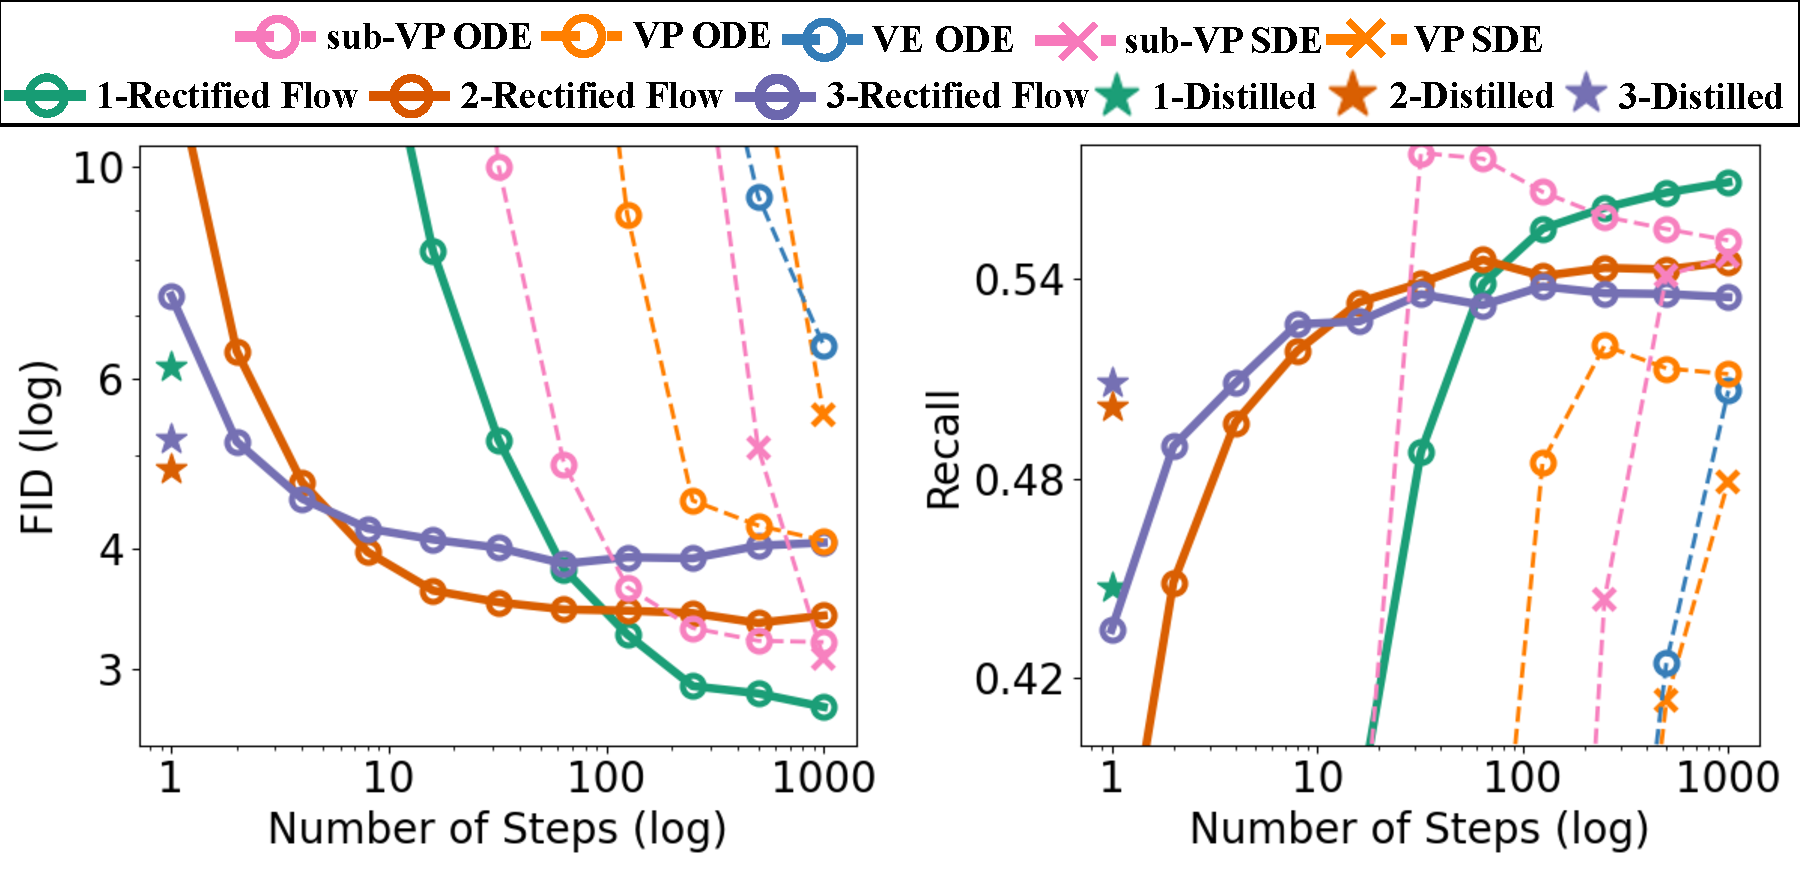
\includegraphics[width=.47\textwidth]{arxiv_figures/fig_cifar_step_method.pdf} & 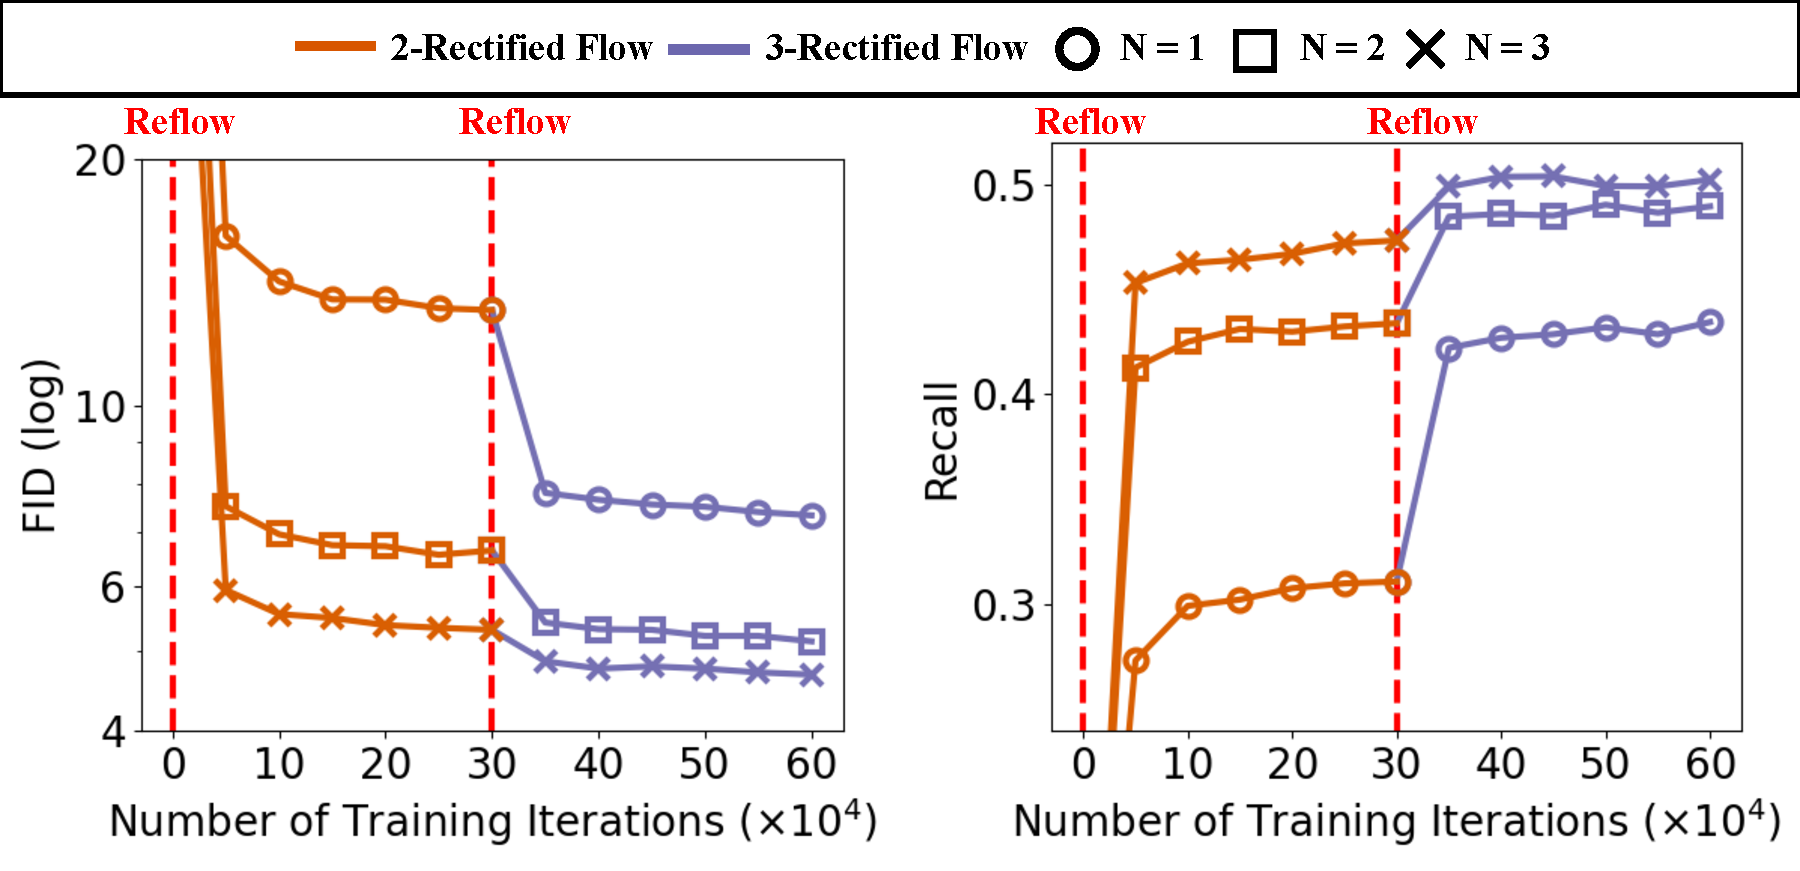
\includegraphics[width=.47\textwidth]{arxiv_figures/fig_cifar_step_123.pdf}
\\
\footnotesize{(a) FID and Recall vs. Number of Euler discretization steps $N$} & \footnotesize{(b) FID and Recall vs. Training Iterations}
 \\
\vspace{-15pt}
\end{tabular}}
\caption{
(a) Results of rectified flows and (sub-)VP ODE on CIFAR10  
with different number $N$ of Euler discretization steps. 
(b) The FID and recall during different reflow and training steps. 
In (a), \emph{$k$-Distilled} refers to the one-step model distilled from \emph{$k$-Rectified Flow} for $k=1,2,3$. 
}
\label{fig:cifar}
\vspace{-5pt}
\end{figure}

\paragraph{Results} 
\emph{$\bullet$~Results of fully solved ODEs.} 
As shown in Table~\ref{tab:cifar10} (a), 
the 1-rectified flow 
trained on the DDPM++ architecture, solved with RK45, 
yields the lowest FID ($2.58$) and highest recall ($0.57$) among all the ODE-based methods.  
In particular, the recall of 0.57 yields a substantial improvement over existing ODE and GAN methods. 
Using the same RK45 ODE solver, rectified flows require fewer steps to generate the images compared with VE, VP, sub-VP ODEs. 
The results are comparable to the fully simulated (sub-)VP SDE, which yields simulation cost. 

\begin{wrapfigure}{r}{0.45\textwidth}
    \vspace{-1\baselineskip}
    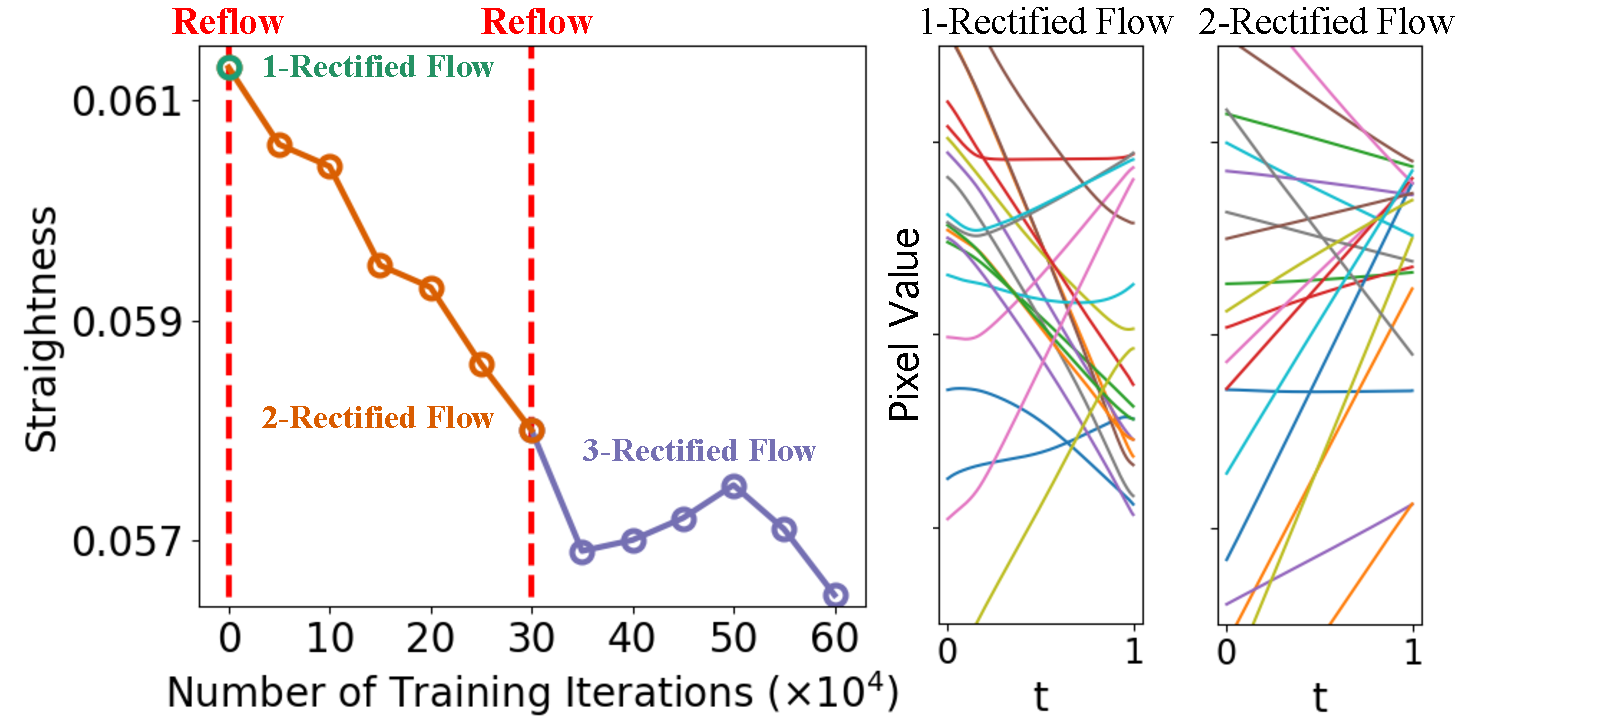
\includegraphics[width=0.48\textwidth]{arxiv_figures/fig_cifar_straightness.pdf}
    \caption{
    The straightening effect on CIFAR10. 
    Left: %
    the straightness measure on different reflow steps and training iterations. 
    Right: trajectories of randomly sampled pixels following 1- and 2-rectified flow. 
    }
    \vspace{-1\baselineskip}
    \label{fig:cifar_straight}
\end{wrapfigure}
\emph{$\bullet$~Results on few and single step generation.} 
As shown in Figure~\ref{fig:cifar}, 
the reflow procedure substantially improves both FID and recall in the small step regime (e.g., $N{\scriptsize\lessapprox}80$), even though it worsens the results 
in the large step regime due to the accumulation of error on estimating $v^x$. 
Figure~\ref{fig:cifar} (b) show that each reflow leads to a noticeable improvement in FID and recall.   
For one-step generation $(N=1)$, 
the results are further boosted by distillation (see the stars in Figure~\ref{fig:cifar} (a)).  
Overall, the distilled $k$-Rectified Flow  with $k=1,2,3$  
yield one-step generative models 
beating all previous ODEs with distillation; 
they also beat the reported results of one-step models with similar U-net type architectures 
trained using GANs (see the \emph{GAN with U-Net} in Table~\ref{tab:cifar10} (b)). 

In particular, 
the distilled 2-rectified flow achieves an FID of $4.85$, beating the best known one-step generative model with U-net architecture, $8.91$ (TDPM, Table~\ref{tab:cifar10} (b)).
The recalls of 
both 2-rectified flow ($0.50$) and 3-rectified flow ($0.51$) outperform the best known results of GANs ($0.49$ from StyleGAN2+ADA)
showing an advantage in diversity. 
We should note that the reported results of GANs have been carefully optimized 
with special techniques such as adaptive discriminator augmentation (ADA)~\citep{karras2020training}, while our results are
based on the vanilla implementation of rectified flow. 
It is likely to further improve rectified flow with proper data augmentation techniques, or the combination of GANs such as 
those proposed by TDPM~\citep{zheng2022truncated} and denoising diffusion GAN~\citep{xiao2021tackling}.







\emph{$\bullet$~Reflow straightens the flow.} 
Figure~\ref{fig:cifar_straight} shows the reflow procedure decreases improves the straightness of the flow on CIFAR10.  
In Figure~\ref{fig:cat_target} visualizes the trajectories of 1-rectified flow and 2-rectified flow on the AFHQ cat dataset: 
at each point $z_t$, we extrapolate the terminal value at $t=1$ by 
$\hat{z}_1^t = z_t + (1-t) v(z_t, t)$; 
if the trajectory of ODE follows a straight line, 
$\hat{z}_1^t$ should not change  as we vary $t$ when following the same path.  
We observe that $\hat{z}_1^t$ is almost independent with $t$ for 2-rectified flow, 
showing the path is almost straight.  
Moreover, even though 1-rectified flow is not straight with $\hat z_1^t$ over time, 
it still yields recognizable and clear images very early ($t\approx 0.1$). 
In comparison,  
it is need $t\approx 0.6$ to get a clear image
from the extrapolation of sub-VP ODE.  



\paragraph{High-resolution image generation}
Figure~\ref{fig:high_res} shows the result of 1-rectified flow on image generation  
on high-resolution ($256 \times 256$) datasets, including  
 LSUN Bedroom~\citep{yu2015lsun}, LSUN Church~\citep{yu2015lsun}, CelebA HQ~\citep{karras2018progressive} to AFHQ Cat~\citep{choi2020stargan}. We can see that it can generate high quality results across the different datasets.  
 Figure~\ref{fig:cat_k} \& \ref{fig:cat_target} show that 
1-(2-)rectified flow yields good results within one or few Euler steps.  

Figure~\ref{fig:interp_editing} shows a simple example of image editing using 1-rectified flow: 
We first obtain an unnatural image $z_1$ by stitching the upper and lower parts of two natural images, 
and then run 1-rectified flow backwards to get a latent code $z_0$. 
We then modify $z_0$ to increase its likelihood under $\tg_0$ (which is $\normal(0,I)$) 
to get more naturally looking variants of the stitched image. %




\begin{figure}
    \centering
    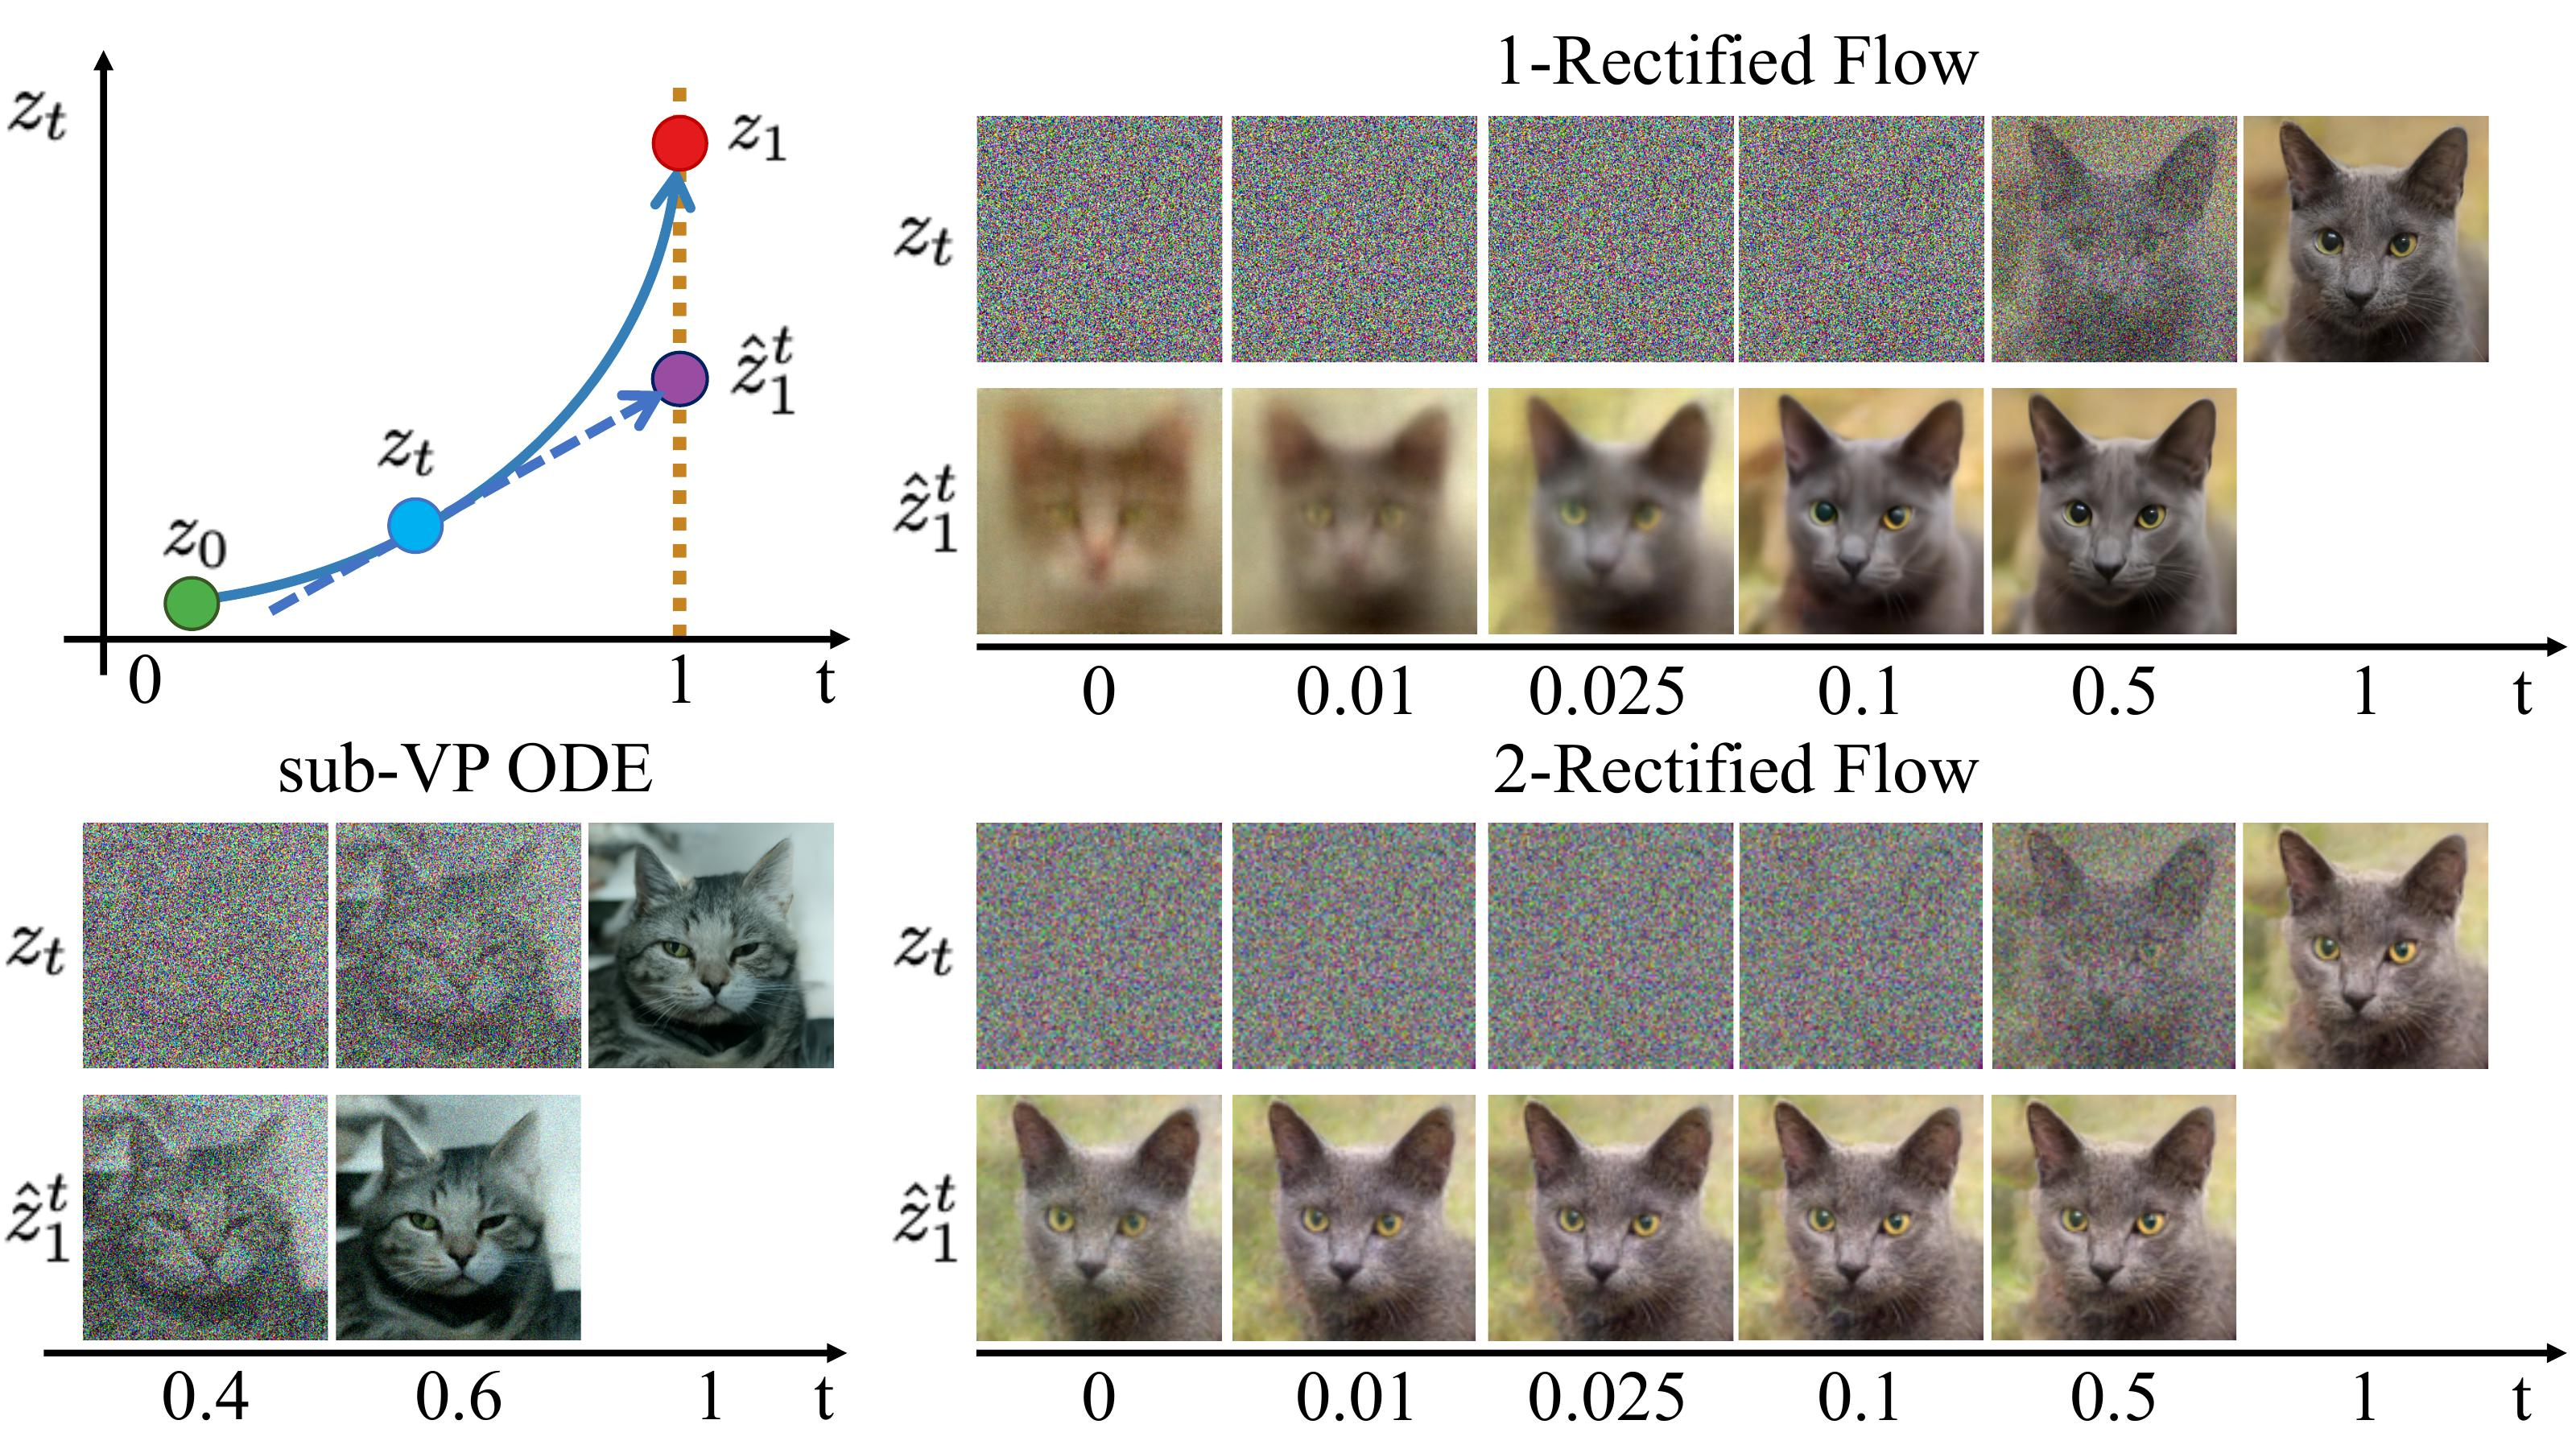
\includegraphics[width=0.9\textwidth]{arxiv_figures/cat_target_new.jpeg}
    \caption{
    Sample trajectories $z_t$ of different flows on the AFHQ Cat dataset,  %
    and the extrapolation $\hat{z}_1^t =z_t + (1-t) v(z_t, t)$ from different $z_t$. The same random seed is adopted for all three methods. The $\hat z_1^t$ of 2-rectified flow is almost independent with $t$, indicating that its trajectory is almost straight. 
    }
    \label{fig:cat_target}
\end{figure}


\begin{figure}
    \centering
    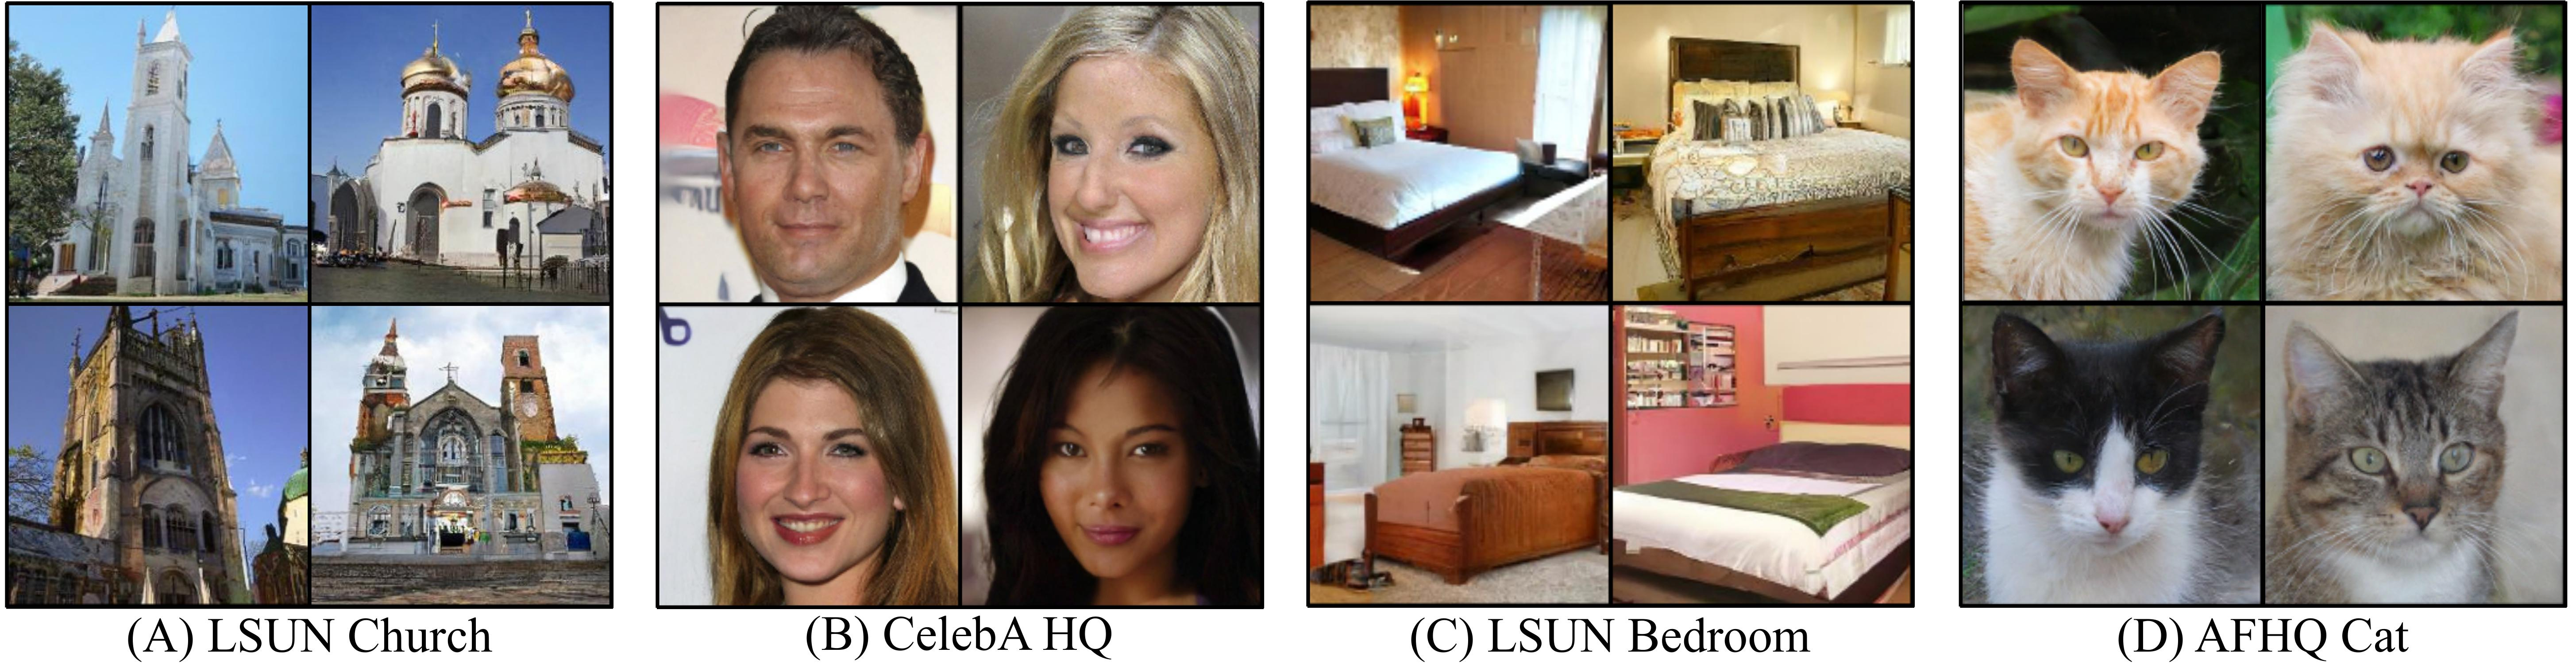
\includegraphics[width=0.95\textwidth]{arxiv_figures/highres.jpeg}
    \caption{Examples of $256\times 256$ images generated by 1-rectified flow.}
    \label{fig:high_res}
\end{figure}


\begin{figure}
    \centering
    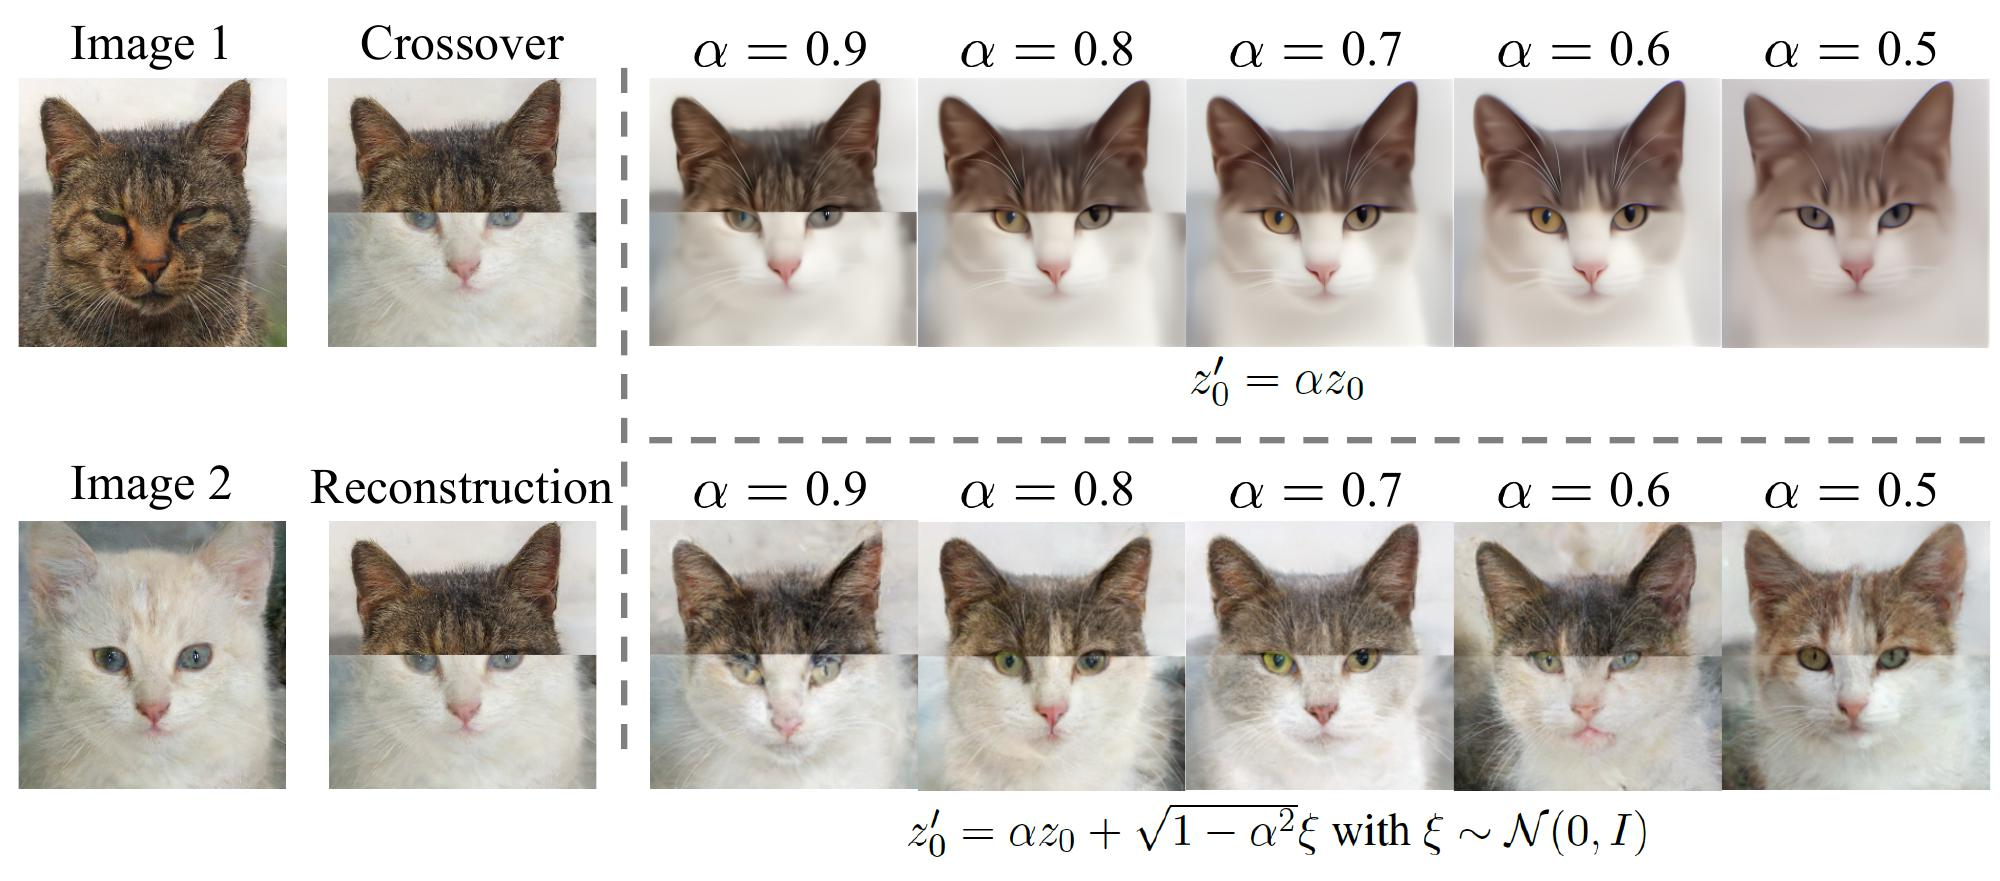
\includegraphics[width=0.95\textwidth]{arxiv_figures/image_editing.jpeg}
    \caption{An example of image editing using 1-rectified flow. 
    Here, we stitch the images of a white cat and a black cat into an unnatural image (denoted as $z_1$).  
    We simulate the  ODE reversely from $z_1$ to get the latent code $z_0$. %
    Because $z_1$ is not a natural image, $z_0$ should have low likelihood under $\tg_0 = \normal(0,I)$.  
    Hence, we move $z_0$ towards the high probability region of $\tg_0$ to get $z_0'$ and solve the ODE forwardly to get a more realistically looking image $z_1'$. 
    The modification can be done deterministically by improving the $\tg_0$-likelihood via $z_0' =\alpha z_0$ with $\alpha\in(0,1)$, or 
    stochastically by  Langevin dynamics, 
    which yields a  formula of 
    $z'_0 = \alpha z_0 + \sqrt{1-\alpha^2}\xi$ with $\xi \sim \normal(0, I)$. 
    }
    \label{fig:interp_editing}
\end{figure}

\begin{figure}[h]
\resizebox{1\textwidth}{!}{
\begin{tabular}{cccc}
     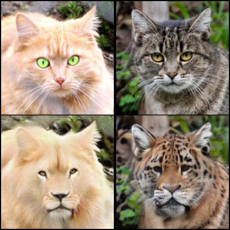
\includegraphics[width=0.23\textwidth]{arxiv_figures/translation_transfer/image_1.png} & 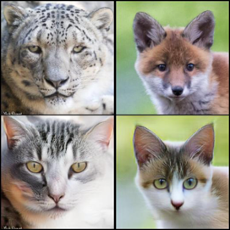
\includegraphics[width=0.23\textwidth]{arxiv_figures/translation_transfer/image_3.png} & %
     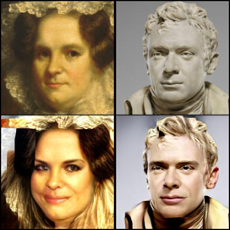
\includegraphics[width=0.23\textwidth]{arxiv_figures/translation_transfer/image_2.png} &%
     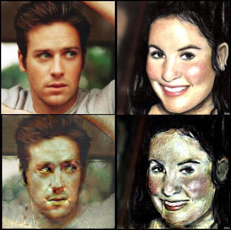
\includegraphics[width=0.23\textwidth]{arxiv_figures/translation_transfer/image_4.png}\\
     \small (A) Cat $\rightarrow$ Wild Animals & \small (B) Wild Animals $\rightarrow$ Cat & \small (C) MetFace $\rightarrow$ CelebA Face & \small (D) CelebA Face $\rightarrow$ MetFace 
\end{tabular}
}
    \caption{
Samples of 1-rectified flow simulated with $N=100$ Euler steps between different domains. 
    }
    \label{fig:met2cat}
\end{figure}

\begin{figure}[h]
\centering
\begin{tabular}{ccccc}
     Initialization & 1-Rectified Flow & 2-Rectified Flow & 1-Rectified Flow  & 2-Rectified Flow\\
     & $N=100$ & $N=100$ & $N=1$  & $N=1$\\
     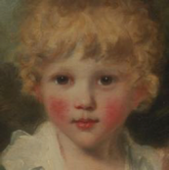
\includegraphics[width=0.16\textwidth]{arxiv_figures/translation_nfe/image_1_1.png} & 
     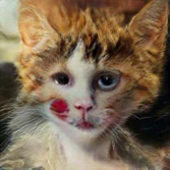
\includegraphics[width=0.16\textwidth]{arxiv_figures/translation_nfe/image_1_2.png} &
     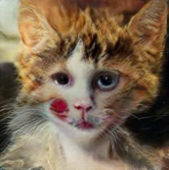
\includegraphics[width=0.16\textwidth]{arxiv_figures/translation_nfe/image_1_3.png} &
     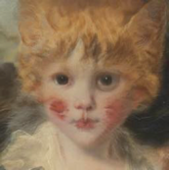
\includegraphics[width=0.16\textwidth]{arxiv_figures/translation_nfe/image_1_4.png} &
     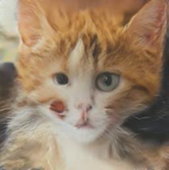
\includegraphics[width=0.16\textwidth]{arxiv_figures/translation_nfe/image_1_5.png}\\
     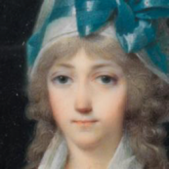
\includegraphics[width=0.16\textwidth]{arxiv_figures/translation_nfe/image_2_1.png} & 
     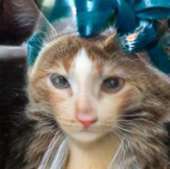
\includegraphics[width=0.16\textwidth]{arxiv_figures/translation_nfe/image_2_2.png} &
     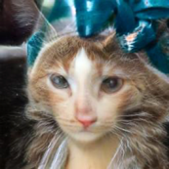
\includegraphics[width=0.16\textwidth]{arxiv_figures/translation_nfe/image_2_3.png} &
     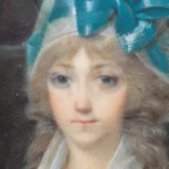
\includegraphics[width=0.16\textwidth]{arxiv_figures/translation_nfe/image_2_4.png} &
     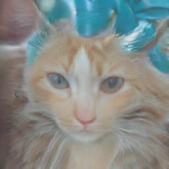
\includegraphics[width=0.16\textwidth]{arxiv_figures/translation_nfe/image_2_5.png}\\
\end{tabular}
    \caption{Samples of results of 1- and 2-rectified flow simulated with $N=1$ and $N=100$ Euler steps.
    }
    \label{fig:met2cat_reflow}
\end{figure}

\subsection{Image-to-Image Translation}


Assume we are given two sets of images of different styles (a.k.a. domains),  
whose distributions are denoted by $\tg_0,\tg_1$, respectively. 
We are interested in transferring the style (or other key characteristics) of the images in one domain to the other domain, in the absence of paired examples. 
A classical approach to achieving this is  
 cycle-consistent adversarial networks (a.k.a. CycleGAN) \citep{cyclegan, isola2017image}, 
 which jointly learns a forward and backward mapping $F,G$ 
 by minimizing the sum of adversarial losses on the two domains, regularized by a cycle consistency loss to enforce $F(G(x))\approx x$ for all image $x$. 

 
By constructing the rectified flow of $\tg_0$ and $\tg_1$,  
we obtain a simple approach to image translation that requires no adversarial optimization and cycle-consistency regularization:  
training the rectified flow requires a simple optimization procedure and the cycle consistency is automatically in  flow  models satisfied due to reversibility of ODEs.  

As the main goal here is to obtain good visual results,  
we are not interested in faithfully transferring $X_0\sim \tg_0$  
to an $X_1$ that exactly follows $\tg_1$. 
Rather, we are interested in 
transferring the image styles while preserving the identity of the main object in the image. For example, 
when transferring a human face image to a cat face, 
we are interested in getting a unrealistic face of human-cat hybrid that still ``looks like" the original human face.

To achieve this, 
let $h(x)$ be a feature mapping of image $x$ representing the styles that we are interested in transferring. 
Let $X_t = t X_1 + (1-t) X_0$. Then $H_t = h(X_t)$ follows an ODE of $\d H_t = \dd h(X_t)\tt (X_1-X_0)\dt .$ Hence, to ensure that the style is transferred correctly, 
we propose to %
learn $v$ such that $H_t' = h(Z_t)$ with $\d Z_t  = v(Z_t,t)\dt $ approximates $H_t$ as much as possible. 
Because $\d H_t' = \dd h(Z_t) \tt v(Z_t, t)\dt$, we propose to minimize the following loss: 
\begin{align}\label{equ:hloss}
    \min_v \int_0^1\mathbb{E} \left[ \norm{ \nabla h(X_t)\tt (X_1 - X_0 - v (X_t, t)) }_2^2 \right ] \dt , && X_t = t X_1 + (1 - t) X_0. 
\end{align}
In practice, we set $h(x)$ to be latent representation of a classifier trained 
to distinguish the images from the two domains $\tg_0,\tg_1$, fine-tuned from a pre-trained ImageNet \citep{tan2019efficientnet} model. %
Intuitively, $\nabla_x h(x)$ serves as a saliency score and re-weights coordinates so that the loss in \eqref{equ:hloss} focuses on penalizing the error that causes significant changes on $h$. 





\begin{figure}[h]
\centering
\setlength{\tabcolsep}{1pt}
\renewcommand\arraystretch{0.4}
\begin{tabular}{cc}
     & \scriptsize{1-Rectified Flow} \\
     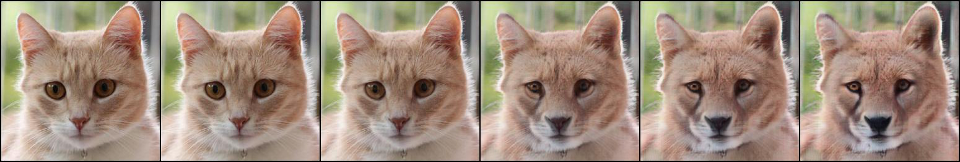
\includegraphics[width=0.48\textwidth]{arxiv_figures/trajectory/image_1.png} &
     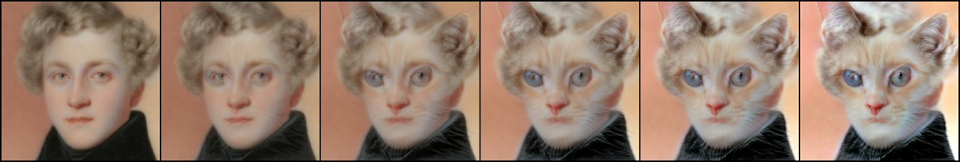
\includegraphics[width=0.48\textwidth]{arxiv_figures/trajectory/image_5.png}
     \\
     & \scriptsize{2-Rectified Flow} \\
     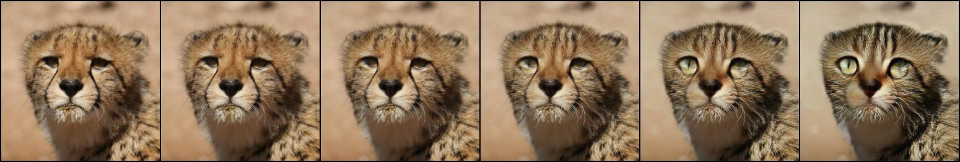
\includegraphics[width=0.48\textwidth]{arxiv_figures/trajectory/image_2.png} & 
     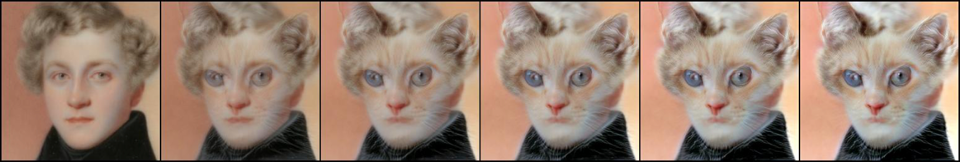
\includegraphics[width=0.48\textwidth]{arxiv_figures/trajectory/image_6.png}
     \\
     & \scriptsize{1-Rectified Flow} \\
     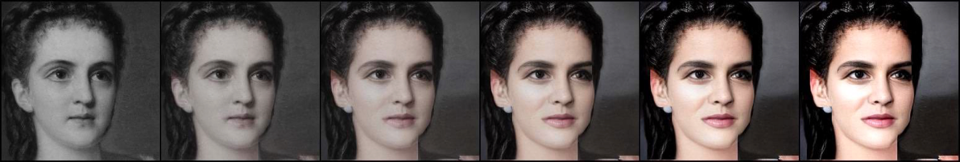
\includegraphics[width=0.48\textwidth]{arxiv_figures/trajectory/image_3.png} & 
     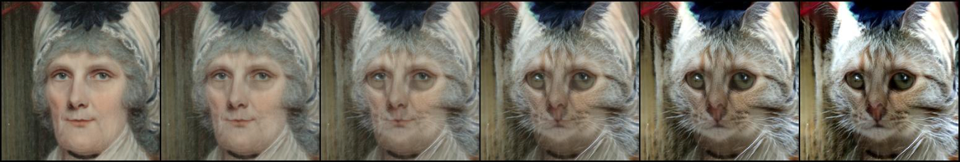
\includegraphics[width=0.48\textwidth]{arxiv_figures/trajectory/image_7.png}
     \\
     & \scriptsize{2-Rectified Flow} \\
     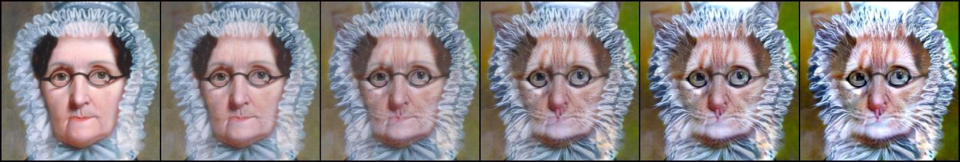
\includegraphics[width=0.48\textwidth]{arxiv_figures/trajectory/image_4.png} & 
     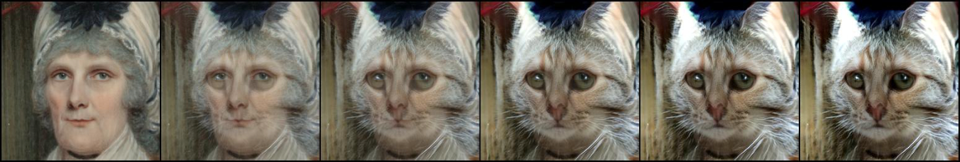
\includegraphics[width=0.48\textwidth]{arxiv_figures/trajectory/image_8.png}
     \\
     \hspace{3pt}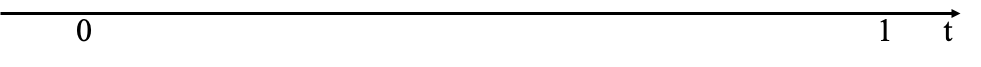
\includegraphics[width=0.485\textwidth]{arxiv_figures/trajectory/axis.png} & 
     \hspace{3pt}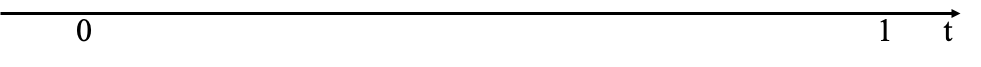
\includegraphics[width=0.485\textwidth]{arxiv_figures/trajectory/axis.png} \\
     (a) 1-rectified flow between different domains & (b) 1- and 2-rectified flow for MetFace $\rightarrow$ Cat.  \\
     
\end{tabular}
    \caption{(a) Samples of  trajectories $z_t$ of 1- and 2-rectified flow for transferring between different domains. }
    \label{fig:met2cat_traj}
\end{figure}

    

\paragraph{Experiment settings}
We set the domains $\tg_0,\tg_1$ to be pairs of 
the AFHQ \citep{choi2020stargan}, MetFace \citep{karras2020training} and CelebA-HQ \citep{karras2018progressive} dataset. 
For each dataset, we randomly select $80\%$ as the training data and regard the rest as the test data; and the results are shown by initializing the trained flows from the test data.
We resize the image to $512 \times 512$.
The training and network configurations  
generally follow the experiment settings in Section~\ref{sec:exp:cifar}. See the appendix for detailed descriptions. 

\paragraph{Results}
Figure~\ref{fig:cat_k}, \ref{fig:met2cat}, \ref{fig:met2cat_reflow}, \ref{fig:met2cat_traj} 
show examples of results of 1- and 2-rectified flow simulated with Euler method with different number of steps $N$.  
We can see that rectified flows can successfully transfer the styles and generate high quality images. 
For example, when transferring cats to wild animals,  
we can generate diverse images with different animal faces, {e.g.}, fox, lion, tiger and cheetah. 
Moreover, with one step of reflow, 2-rectified flow returns good results with a single Euler step ($N=1$).  
See more examples in Appendix. 



\subsection{Domain Adaptation} 
A key challenge of applying machine learning  to  real-world problems is the domain shift between the training and test datasets: the performance of machine learning models may degrade significantly 
when tested on a novel domain different from the training set.  
Rectified flow can be applied to transfer the novel domain ($\tg_0$) to the training domain ($\tg_1$) to mitigate the impact of domain shift. 

\paragraph{Experiment settings} We test the rectified flow for domain adaptation on 
a number of datasets. 
DomainNet \citep{peng2019domainnet} is a dataset of common objects in six different domain taken from DomainBed  \citep{gulrajani2020search}. %
All domains  from DomainNet  include 345 categories (classes) of objects such as Bracelet, plane, bird and cello. 
Office-Home \citep{venkateswara2017officehome} is a benchmark dataset for domain adaptation which contains 4 domains where each domain consists of 65 categories. 
To apply our method, 
first we map both the training and testing data 
to the latent representation from final hidden layer of the pre-trained model, and construct the rectified flow on the latent representation. 
We use the same DDPM++ model architecture %
for training. %
For inference, we set the number of steps of our flow model as $100$ using uniform discretization.
The methods are evaluated by the prediction accuracy of the transferred testing data 
on the classification model trained on the training data. 

\paragraph{Results}
As demonstrated in Table \ref{tab:domainbed}, 
the 1-rectified flow shows  
state-of-the-art performance 
on both DomainNet and OfficeHome. 
It is better or on  par with 
the previous best approach (Deep CORAL \citep{sun2016coral}), 
while sustainably improve over all other methods.



\begin{table}[]
    \centering
    \scalebox{0.88}{
    \begin{tabular}{l|cccccc|c}
    \hline
        Method & ERM & IRM & ARM & Mixup & MLDG & CORAL & Ours\\
        \hline
        OfficeHome & $66.5\pm0.3$ & $64.3\pm2.2$ & $64.8\pm0.3$ & $68.1\pm0.3$ & $66.8\pm0.6$  & $68.7\pm0.3$  & $\bf 69.2\pm0.5$ \\
        DomainNet & $40.9\pm0.1$ & $33.9\pm2.8$ & $35.5\pm0.2$ & $39.2\pm0.1$ & $41.2\pm0.1$ & $\bf 41.5\pm0.2$ & $\bf 41.4\pm0.1$ \\
    \hline
    \end{tabular}}
    \caption{The accuracy of the transferred testing data using different methods, on the OfficeHome and DomainNet dataset. 
    Higher accuracy means the better performance. }
    \label{tab:domainbed}
\end{table}


    

    


    

    


